%# -*- coding: utf-8-unix -*-
%%==================================================
%% chapter01.tex for SJTU Master Thesis
%%==================================================

%\bibliographystyle{sjtu2}%[此处用于每章都生产参考文献]
\chapter{混合存储系统设计中的关键技术研究}
\label{chap:key_tech}

目前,针对基于SDD与HDD的混合存储系统的设计主要从系统架构、数据映射策略、冷热数据识别策略、数据写回/迁移策略、最优化存储设备组合这五个方面展开。

\section{系统架构}

目前基于SSD与HDD的混合存储系统主要有两种系统架构:一种是分层的架构,将SSD作为HDD的缓存;另一种是同层的架构,将SSD与HDD放在同一层,对存储系统而言,SSD与HDD是相对独立的存储设备。

\subsection{分层架构}

分层架构的结构如图\ref{fig:multi_layer_architecture}所示,在该架构下,SSD被完全用作HDD的缓存,混合存储系统的逻辑地址与HDD的物理地址一一对应,当混合存储系统收到来自上层的I/O请求时,首先在SSD中找寻是否存在该数据,如果存在该数据则直接在SSD中对该数据进行操作,否则会去访问HDD进行进一步操作。

在分层架构下,由于SSD比RAM以及NVRAM有更大的容量,因此较RAM与NVRAM可以缓存更多数据,使得系统整体的命中率得到提升,进而提升系统整体的读写性能。然而该架构下仍然要面临被缓存在SSD中的脏数据的处理问题,即是频繁缓存到SSD中提高性能还是频繁写回到HDD中提升SSD的寿命这一两难问题。

\begin{figure}[!htp]
    \centering
    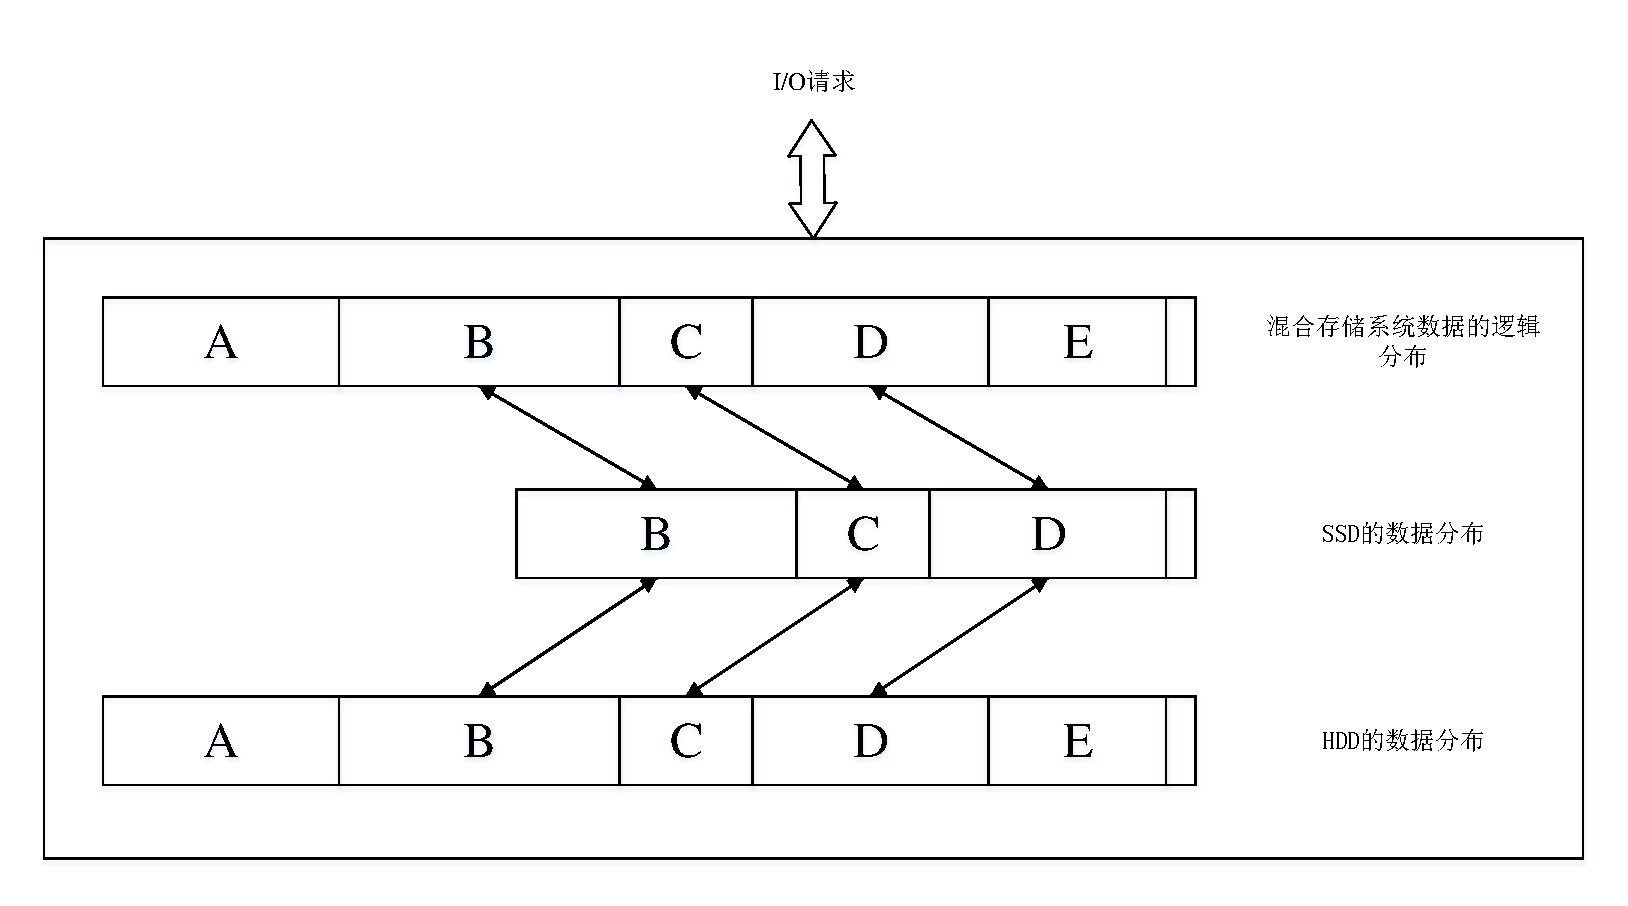
\includegraphics[width=0.8\textwidth]{multi_layer_architecture.pdf}
    \bicaption[fig:multi_layer_architecture]{分层混合存储系统架构}{分层混合存储系统架构}{Fig}{multi-layer hybrid storage system architecture}
\end{figure}

\subsection{同层架构}

分层架构的结构如图\ref{fig:single_layer_architecture}所示,在该架构下,SSD与HDD处于同一层,混合存储系统的逻辑地址为SSD的物理地址与HDD的物理地址之和,当混合存储系统收到来自上层的I/O请求时会根据逻辑地址直接去找到实际存储设备的物理地址进行数据访问,但是系统会根据数据的冷热程度不同对数据进行迁移,将热数据放到SSD上而将冷数据放到HDD上。

在同层架构下,系统的整体容量为SSD与HDD的容量之和,相比分层架构提高了容量的利用率,同时根据数据冷热程度不同放到不同的存储设备上提高了系统整体的性能,但是该架构下系统的实现复杂度会较分层架构提高,同时数据的迁移过程以及数据的冷热识别会直接影响系统的性能。

\begin{figure}[!htp]
    \centering
    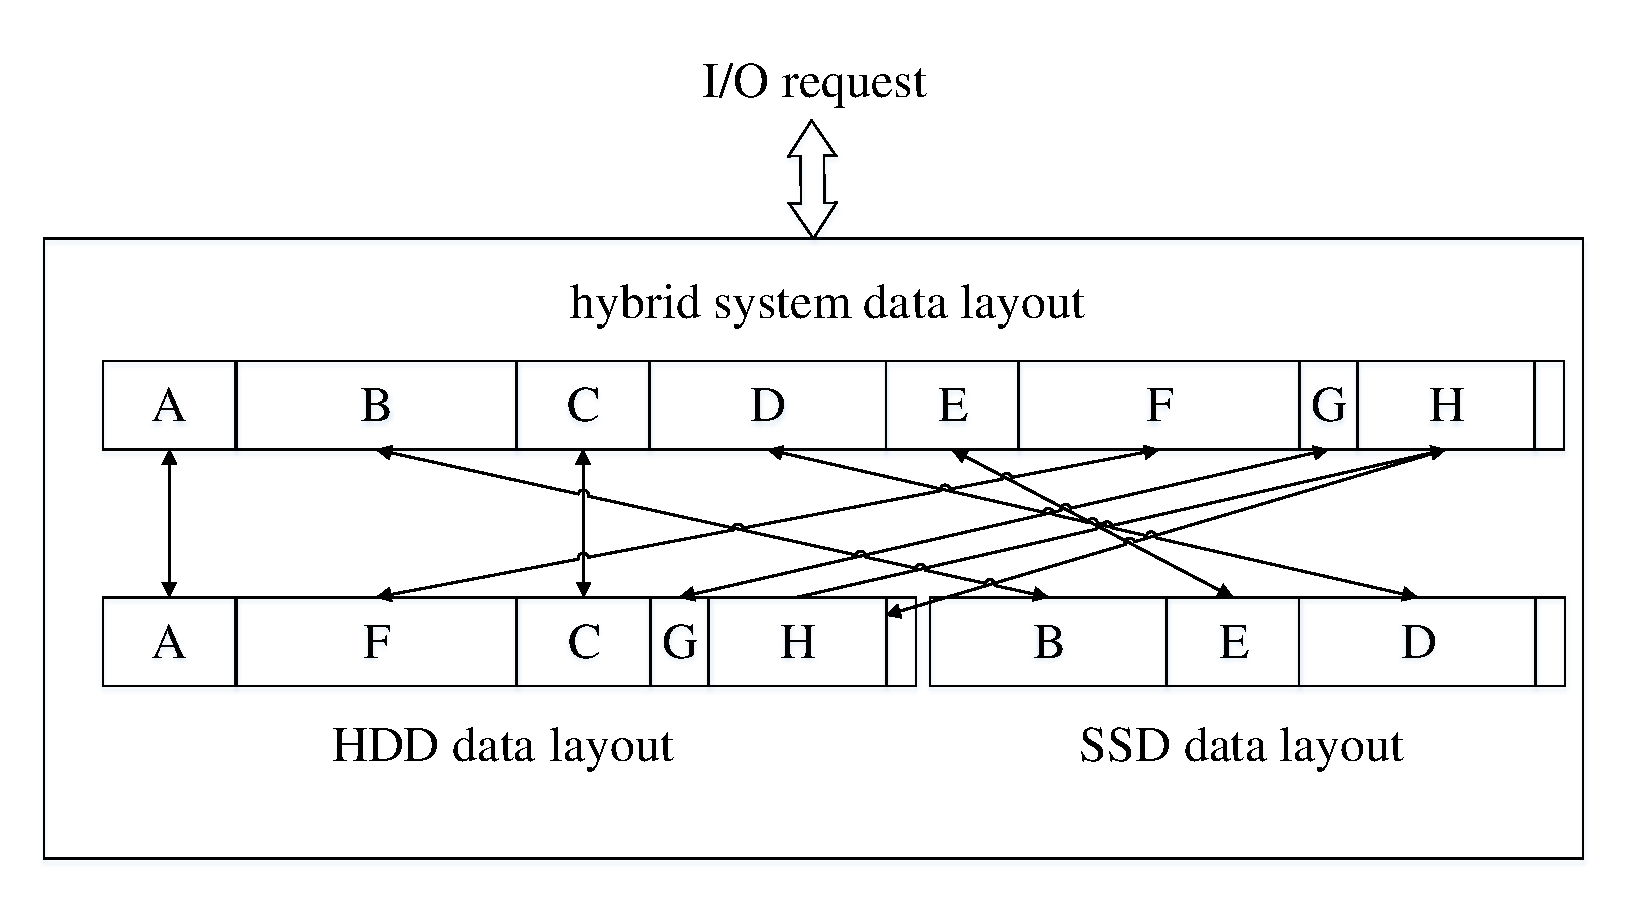
\includegraphics[width=0.8\textwidth]{single_layer_architecture.pdf}
    \bicaption[fig:single_layer_architecture]{同层混合存储系统架构}{同层混合存储系统架构}{Fig}{single-layer hybrid storage system architecture}
\end{figure}

\section{数据映射策略}

无论混合存储系统是分层架构还是同层架构,最后的数据都是以block为单位存放到实际设备上,因此对于每个block的I/O请求需要将其映射到具体的真实设备,这就需要考虑映射的粒度问题与映射的规则。

映射粒度是指在混合存储系统中系统能操作的数据的最小单位,它可以只是一个block的大小,也可以是多个block的大小,但应保证是block大小的整数倍。一般而言,映射粒度分为block级、文件级与Extent级三个级别。映射规则是指混合存储系统中的逻辑地址与实际设备的物理地址的转换规则。一般而言,映射规则分为纯计算类型、依靠映射表类型与计算和映射表混合类型三种。

\subsection{块级映射策略}

块级映射即以4KB的块(block)为操作数据的最小单位。所有的实际设备以4KB为大小划分为多个block,对混合存储系统中的每个block的I/O请求依照特定映射规则,映射到具体的实际设备进行实际操作。一般而言,块级映射策略用于分层架构的混合存储系统中,其映射规则与高速缓存和主存的映射规则类似,可分为全相联、直接映射和组相联三种。全相联即是指HDD的任一block可以映射到SSD的任一block,直接映射是指HDD的第j块block只能映射到满足如下特定关系的SSD的第i块block中($i=j mod SSD的block数$)。组相联则是结合了全相联与直接映射,首先将多个block组成一个组,HDD的组与SDD的组之间采用直接映射的方式,而组内部的块则采用全相联的方式映射。

块级映射的映射策略较为简单,且可以以最细的粒度对数据进行操作,但是粒度越细,系统的额外开销也就越大。虽然HDD映射到SSD时可以通过直接映射的方式避免映射表,但是当需要将SSD的数据写回到HDD时势必需要一张映射表才能找到正确的位置。假设SSD的容量为100GB,映射表的每个block对应的表项的大小为20bytes,那么整个映射表的大小约为500MB,并且由于映射表是频繁访问的数据,需要驻留在内存中,因此最终整个系统需要500MB的额外内存开销,这对普通用户而言属于不可接受的额外开销大小。另外对于顺序读写请求,实际这些请求无论是全部放在SSD上进行或者都放在HDD上进行性能都相差不多,但块级映射可能会将顺序读写请求中的一些数据映射到SSD上另一些则映射到HDD上,最终导致顺序读写请求被分散到SSD和HDD上变成两个随机读写请求,这会极大影响性能。此外,在分层架构中,多个HDD的block会被映射到SSD的同一个block上,那么当发生碰撞时的替换策略对系统的性能影响也很大。

\subsection{文件级映射策略}

文件级映射即以文件为组织block的最小操作单位,同一个文件中的不同block会被映射到同一个设备上,同样,对数据的冷热识别、缓存的最小单位、数据迁移的最小单位也都是文件。相比块级映射,文件级映射的粒度显然粗很多,因此系统的额外开销会小很多,但是由于文件的大小不一,可能会存在很大的文件,当这些文件在分层架构中被缓存需要写回时或者在同层架构中需要被迁移时,系统的负载会一下子增高,而不像块级映射会比较平稳。

\subsection{Extent级映射策略}

Extent级映射即将多个block组成一个extent,以extent作为最小的操作单位,同一个extent中的block会被映射到同一个设备上。与文件级映射不同,同一个文件的block在物理存储上可能不连续,而Extent级映射则通常是将物理连续的多个block组成一个extent。extent的大小可以自由指定,这就让Extent级映射变得很灵活,但同时extent的大小十分讲究,如果设定的太小,那么系统的额外开销就会增加,同时也可能会有顺序读写性能下降的问题,而如果设定的太大,那么系统在冷热数据的识别上就会不精确,并且同样会在写回或者迁移上造成系统的负载瞬间增高。

\section{冷热数据识别策略}

冷热数据识别策略负责将数据区分为冷数据与热数据,提供将需要访问的数据放在高速设备上而将不经常访问的数据放在低速设备上的依据。冷热数据识别策略直接决定数据是否能被存在与其访问频度相符的设备上,因此冷热数据识别的准确性会直接影响系统的整体性能,冷热识别策略可大致分为块级冷热识别策略与文件/Extent级冷热识别策略,下面将分别介绍。

\subsection{块级冷热识别策略}

块级冷热识别策略是粒度最细的冷热识别策略,以块为冷热程度统计的最小单位。块级冷热识别策略将访问频率高的块标记为热数据,其他的标记为冷数据,由于SSD的写前擦除与擦除次数限制的特性,块级冷热识别策略在SSD的内部设计中经常有被应用以使SSD中不同块的负载均衡,使不同块的擦除次数保持平衡。

块级冷热识别策略的优势在于它真正识别出了哪些数据块是最热的数据。但是它只是给出了微观的最优解,但在宏观上未必是最优的。比如对于一组顺序读或顺序写请求,可能这组请求中涉及的数据块有的是冷数据有的是热数据,那么它们就会被存放在不同设备上,使得原本的顺序请求会被打散为在不同设备上的随机请求,这反而会降低系统的性能。

块级冷热识别的算法有很多,经典的有FIFO、LRU等算法,近年来也有ARC\cite{megiddo2003arc}、Clock-Pro\cite{jiang2005clock}、多哈希函数\cite{hsieh2006efficient}、多布隆过滤器\cite{park2011hot}、WDAC\cite{park2011hot}等算法。经典的FIFO、LRU算法虽然计算简单、实现简单,但是热点识别的准确率不高,比如当发生一个很长的循环遍历时,FIFO或者LRU的队列或者链表会被反复替换,导致系统的性能下降。ARC等新算法则通过使用新近性和频度来判断数据的冷热程度,虽然增加了额外的开销和提高了实现的复杂度,但是提高了热点识别的准确率,并且能够抵抗循环遍历造成的热点冲刷。

\subsection{文件/Extent级冷热识别策略}

文件/Extent级冷热识别策略以文件或者Extent为冷热程度统计的最小单位。每个块的I/O请求都会影响该块所属的文件或Extent的热度,同时除了文件或Extent中块的访问频率,该粒度下还可引入文件或Extent中热点块的分布、带宽等更宏观的指标来对更新文件或Extent的冷热程度。

文件/Extent级冷热识别策略的优势在于与块级冷热识别策略相比,更粗的粒度能带来更小的系统额外开销,并且可以同时从微观与宏观两个方面进行热点识别,能够识别出顺序读写请求与随机读写请求,以此为依据避免将顺序读写请求打散到不同设备上。

\section{数据写回/迁移策略}

在混合存储系统中最理想的情况是将热数据都存放在高速设备上,而将冷数据放在低速设备上,但由于数据的冷热程度会不断变化,并且高速设备的容量有限可能并不能存放所有热数据,因此会发生数据不处在与其冷热程度匹配的设备的情况,数据写回/迁移策略就是负责将数据迁移到与其冷热程度匹配的设备上,以提高系统整体的性能。数据写回/迁移策略需要考虑哪些数据需要写回/迁移、何时写回/迁移这些数据、在数据迁移中如何保证系统对外性能这三个问题。

写回/迁移数据的选择根据冷热识别策略决定,一旦冷热识别算法确定,通过该算法就能直接确定哪些热数据处在低速设备上,哪些冷数据处在高速设备上,针对这些数据再以对应的粒度:块级、文件级、Extent级生成待写回/迁移的数据集合即可。

数据的写回/迁移时机大致可分为静态与动态两种策略。静态策略是指系统周期性地对数据进行写回或迁移,静态策略一般选择在系统负载轻的时候(如半夜之后)进行大规模的写回/迁移,因此系统的性能波动对外影响较小,但是静态策略无法及时针对数据的冷热变化作出响应,无法实时达到系统的理论最大性能。动态策略是指不定期地对数据进行写回或迁移以对数据的冷热变化作出实时响应,动态策略可以保证系统的性能一直保持尽可能高,但是动态策略可能会让系统的性能波动变大,并且在系统重负载时影响到对外性能,尤其是当粒度为文件/Extent级时,甚至可能导致系统对外表现为不可用的状态。

\section{最优化存储设备组合}

最优化存储设备组合是指在保证系统达到性能需求的前提下尽可能降低系统的成本,这也是混合存储系统设计中要考虑的问题。该问题需要考虑系统架构、系统负载类型、存储设备的特性等诸多因素。该问题的解决可分为静态策略与动态策略两种。

\subsection{静态策略}

静态策略是指在构建混合存储系统的时候就选取好不同存储设备的型号、数量等,在混合存储系统上线运行后就不再变更,如果需要变更,则需要先将系统停止后更改配置再运行。目前静态策略的生成分为通过模拟\cite{guerra2011cost}给出最优解与通过理论推导计算\cite{kim2011hybridstore}给出最优解两种。

\subsection{动态策略}

动态策略是指在混合存储系统运行过程中能够不需要停止运行就能重新适应用户的新需求,比如在系统运行的过程中对存储设备的热插拔,在系统运行过程中冷热数据识别策略或者数据写回/迁移策略的动态变更等等。

\section{本章小结}

本章主要介绍了混合存储系统设计中的关键问题。首先介绍了系统架构,对分层架构和同层架构进行了阐述;然后介绍了数据映射策略,对块级、文件级、Extent级三种不同映射策略进行了简单的介绍与对比分析;之后介绍了冷热数据识别策略;然后介绍了数据写回/迁移策略,对静态与动态两种策略进行了简单的对比分析;最后介绍了最优化存储设备组合。